\section{Durchführung}
\label{sec:durchfuehrung}

    Im Folgenden sollen nun der Aufbau des Experiments,
    sowie die Durchführung beschrieben werden.

\subsection{Versuchsaufbau}

    Der Gesamtaufbau besteht aus einer \textbf{Rubidium-Spektrallampe},
    welche Licht auf einen Kolben mit Rubidium-Gas strahlt,
    wobei der Kolben von \textbf{Helmholtzspulen} umgeben ist,
    welche verschiedene Magnetfelder erzeugen.
    Das entstehende emittierte Licht wird von einer \textbf{Photozelle} detektiert.
    \autoref{fig:aufbau} zeigt den Aufbau der Apparatur.
    \begin{figure}
        \centering
        \includegraphics[width=\textwidth]{content/img/Abb_1.pdf}
        \caption{Versuchsaufbau mit Spektrallampe, optischen Elementen, Gaskolben und Photoelement in Draufsicht. \cite{versuchsanleitung}}
        \label{fig:aufbau}
    \end{figure}

    Wie in \autoref{sec:theorie:optisches_pumpen} erläutert,
    soll nun rechts polarisiertes Licht mit der Wellenlänge des $D_1$-Übergangs verwendet werden.
    Dazu sind verschiedene optische Elemente gegeben:
    Mithilfe von \textbf{plan-konkaven Sammellinsen} soll der entstehende Lichtstrahl fokussiert werden.
    Da die Rubidium-Lampe nicht nur die $D_1$-Linie erzeugt,
    werden alle anderen Wellenlängen durch einen \textbf{Fabry-Pérot-Etalon} herausgefiltert.
    Anschließend wird der Lichtstrahl mithilfe eines \textbf{Polarisationsfilters} erst linear,
    dann mithilfe eines \textbf{$\sfrac{\lambda}{4}$-Plättchens} zirkular polarisiert.

    Eine \textbf{Heizung} hält das Rubidium in der \textbf{Dampfzelle} auf optimalem Druck.

    Um die Dampfzelle herum sind verschiedene Spulen angeordnet:
    Die größten Beiträge zum Magnetfeld liefern eine \textbf{vertikale Spule} und eine \textbf{horizontale Spule},
    wobei letztere mit einer weiteren Spule, der \textbf{Sweep-Spule}, umwickelt ist.
    Diese erlaubt das periodische Durchlaufen verschiedener Magnetfeldstärken in einer festen Zeit
    (in der Größenordnung von Sekunden).
    Das Magnetfeld dieser Spulen ist über den Stromfluss regelbar.
    %
    Zusätzlich ist eine \textbf{Modulationsspule} eingebaut,
    welche ein radiofrequentes Magnetfeld erzeugt,
    dessen Frequenz am \textbf{HF-Generator} verstellbar ist.

    Mithilfe eines \textbf{Oszilloskops} kann die registrierte Lichtintensität
    in Abhängigkeit vom Magnetfeld der Sweep-Spule (\textit{XY-Modus})
    dargestellt werden.

\subsection{Einjustierung und Kompensation des Erdmagnetfelds}
\label{sec:durchfuehrung:einjustierung}

    Zu Beginn müssen die optischen Elemente im Strahlengang so justiert werden,
    dass die gemessene Intensität maximal wird.
    Es werden dazu erst die beiden Linsen nacheinander in horizontaler und vertikaler Richtung ausgerichtet
    und anschließend die verschiedenen Filter eingebaut.
    Danach wird die Apparatur mit einer Decke abgedeckt,
    damit möglichst wenig äußeres Licht auf die Photozelle trifft.

    Auf dem Oszilloskop ist nun ein breiter Peak zu sehen.
    Als nächstes muss die Vertikalkomponente des Erdmagnetfelds kompensiert werden.
    Dazu wird der Stromfluss durch die Vertikalspule mithilfe eines Potentiometers so erhöht,
    dass der Peak möglichst schmal wird.

    Um die Horizontalkomponente zu kompensieren,
    wird der Tisch, auf dem die Apparatur steht, so gedreht,
    dass der Strahlengang in Nord-Süd-Richtung ausgerichtet ist.
    Auch hier soll der Peak möglichst schmal werden.

\subsection{Messung der Magnetfeldstärke der Rubidium-Isotope} %TODO: komische Bezeichnung
\label{sec:durchfuehrung:messung}

    Für diese Messung wird zum ersten Mal ein Strom durch die Modulationsspule geleitet,
    welcher sinusförmig ist und eine Frequenz $f$ hat.
    Diese Frequenz wird in der folgenden Messung von \SI{100}{\kilo\hertz} an in Schritten von \SI{100}{\kilo\hertz} bis auf \SI{1000}{\kilo\hertz} erhöht.

    Bei einer Frequenz von \SI{100}{\kilo\hertz} und unter Verwendung der Sweep-Spule ergibt sich eine Darstellung wie in \autoref{fig:peaks},
    welche während der Messung aufgenommen wurde.
    \begin{figure}[H]
       \centering
       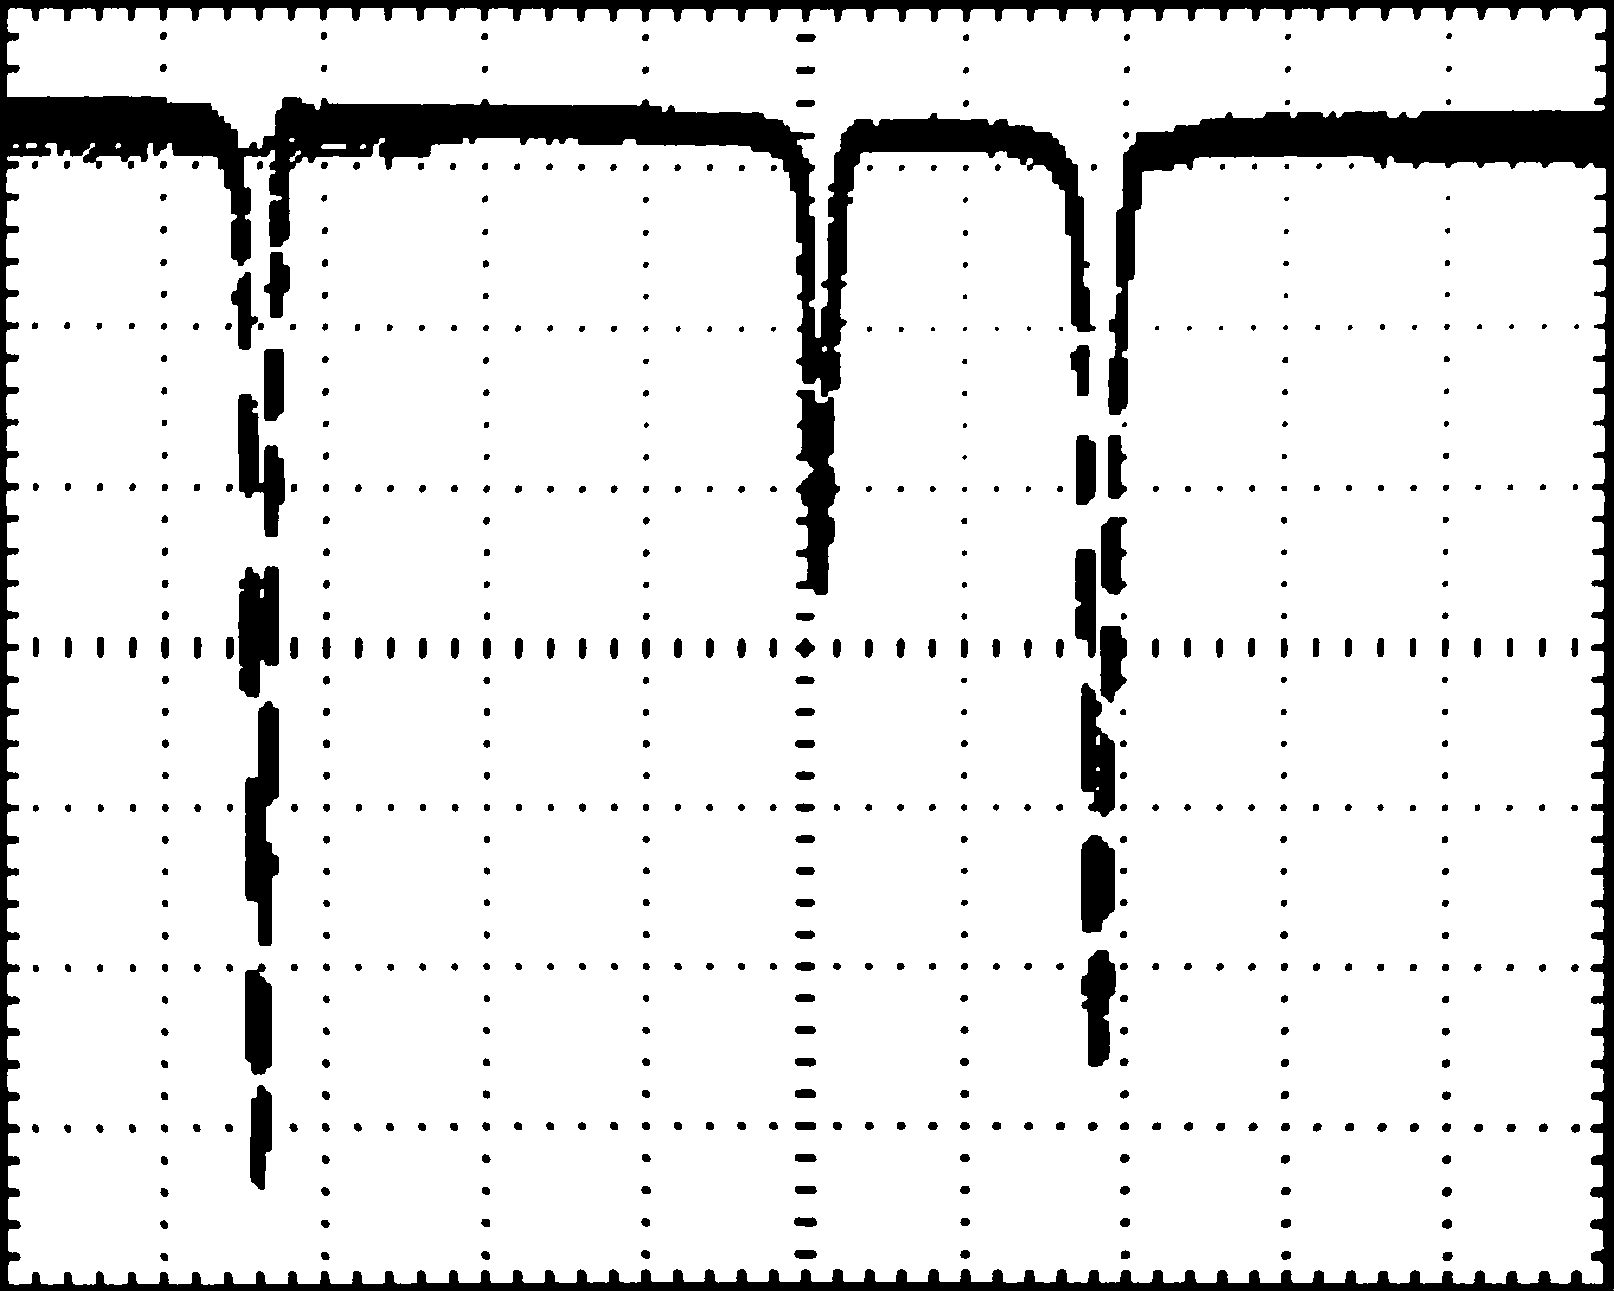
\includegraphics[width=0.5\textwidth]{content/img/oszilloskop1.png}
       \caption{
            Bildschirmfoto des Oszilloskops bei $f = \SI{100}{\kilo\hertz}$.
            In der Abszissenachse ist der Sweep-Spulenstrom, in der Ordinatenachse die gemessene Lichtintensität aufgetragen.
        }
       \label{fig:peaks}
    \end{figure}

    Der größte Peak entspricht $B_\text{ges} = \SI{0}{\tesla}$;
    etwa dort beginnt anfangs der Sweep.
    Die beiden kleineren Peaks rechts stammen von den Resonanzen der Rubidium-Isotope.
    Sie sind nur vom Betrag des äußeren Magnetfelds abhängig und daher symmetrisch um den \enquote{$B=0$}-Peak angeordnet.
    Es genügt also – wie in der Abbildung – nur eine Seite zu vermessen.

    Das Oszilloskop wird nun so eingestellt,
    dass mit Erhöhen der Stromstärke in der horizontalen Sweep-Spule der Verlauf der Kurve mithilfe eines anderen Potentiometers abgelaufen werden kann,
    wobei jeweils der Stromwert notiert wird,
    für den die Spitze eines der Isotopen-Peaks erreicht wird.
    Sollte die Feldstärke der Sweep-Spule zum Erreichen der Peaks nicht ausreichen,
    kann die Stromstärke in der horizontalen Spule erhöht werden.
    Der Gesamtwert des entsprechenden Magnetfelds ergibt sich aus Summation der Magnetfelder beider Spulen.
    Diese Messung wird für jede Frequenz aus dem oben genannten Bereich wiederholt.

    Zuletzt wird für eine Frequenz von \SI{100}{\kilo\hertz} die Amplitude der beiden Isotopen-Peaks auf dem Oszilloskop vermessen.
